%\label{sec:statistical_framework}

\subsection{Fitting Framework}

The fitting framework is based on XML Analytic Workspace Builder~\cite{xmlAnaWSBuilder} (xmlAnaWSBuilder) 
which is widely used in the Higgs Group. XmlAnaWSBuilder creates RooFit~\cite{RooFit} workspaces using one-dimensional 
observables and its workflow of the framework is summarised in Fig.~\ref{fig:xmlAnaWSBuilderworkflow}.

\begin{figure}[htb]
 \centering
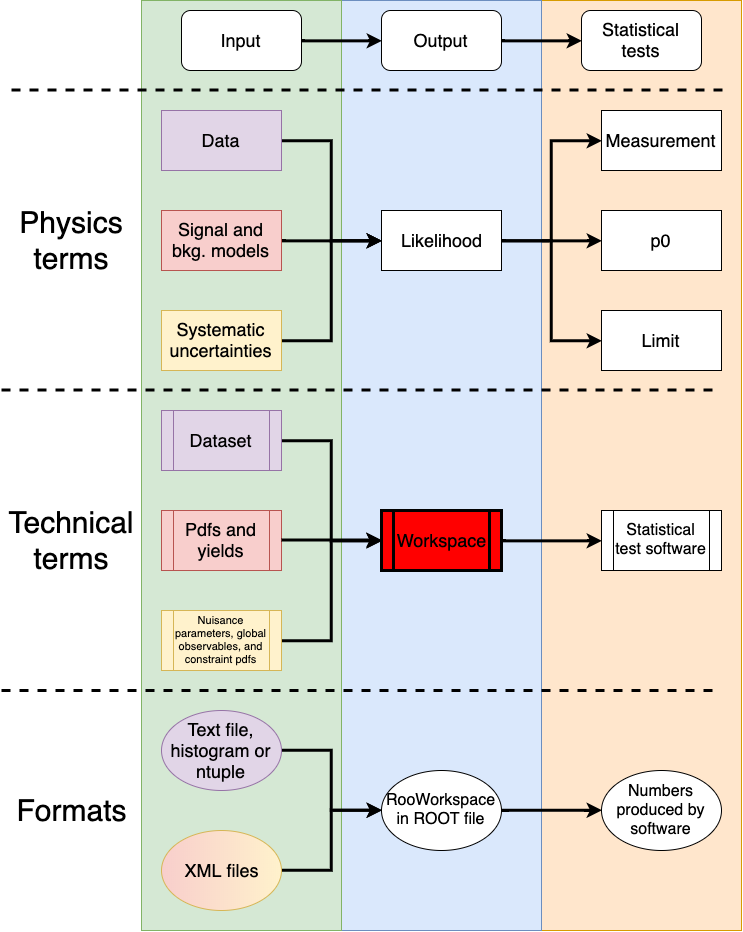
\includegraphics[width=0.75\textwidth]{figures/06-StatisticalFramework/xmlAnaWSBuilder_workflow}
\caption{The XmlAnaWSBuilder workflow.  \label{fig:xmlAnaWSBuilderworkflow}}
\end{figure}

The data fitting will use the quickFit framework~\cite{quickFit} with modifications to allow for integrating over binned data.
RooFit evaluates it's fit functions at the centre of each bin rather than at the center of gravity. This leads to significant 
biases in the fit results ~\cite{gligorov2021avoiding} which are very large with steeply falling data spectra like the dijet mass. 
Recent developments in RooFit have created a new class, \texttt{RooBinSamplingPdf}, can now be used to avoid this problem 
which is available in a patch to ROOT v6.23~\cite{RooBinSamplingPdf} and built in the v6.24 release. 


\subsection{Background Estimation}

In the resonant search the SM background of the \mjj\ spectrum is determined by a functional fit to the data.
Previous searches, from ATLAS and other experiments (such as Refs.~\cite{Bagnaia:1984ip,PhysRevD.79.112002,EXOT-2010-01,CMS-EXO-10-010,EXOT-2010-07,EXOT-2013-11})
have found that a parametric function of the form
\begin{equation}
  f(x) = p_1 (1 - x)^{p_2} x^{p_3 + p_4\ln x + p_5 (\ln x)^2},
%\label{Eq:fitfunction}% uncomment if label used. 
\end{equation}
where $x \equiv \mjj /\sqrt{s}$, accurately describes dijet mass distribution predicted by leading and next-to-leading-order 
QCD Monte Carlo. In the ATLAS Run~2 analysis with \integLumi\ of data  \cite{EXOT-2019-03,Nishu:2646455}. the four parameter 
version of the function was found to properly describe the QCD background ($p_5 = 0$) function sufficiently described the data.  
The introduction of  gluon tagging may require more  parameters to properly describe the full invariant mass spectrum.
\todo[inline]{Is the fifth term $(\ln x)^2$ or $x$? }

To ensure the removal of biases from the creation of pseudo data and as a cross check we require an alternative functional 
form which is based on that used by UA2 \cite{Alitti:1990kw, Alitti:1993pn} in its observation of the $W$ and $Z$ decaying 
to two jets and subsequent search
\begin{equation}
  f(x) = p_1 x^{p_2} \exp\left({p_3 x + p_4  x^2 }\right).
%\label{Eq:fitfunction2}% uncomment if label used. 
\end{equation}
